\section{Evaluation and Benchmark Analysis}
\label{sec:evaluation-benchmark-analysis}

Evaluation is the central bottleneck of AI self-evolution. A self-evolving system is defined not merely by the fact that it changes, but by the claim that its changes are improvements. That claim is always mediated by an evaluator: a unit test, a hidden benchmark, a reward model, a formal verifier, a human preference, a simulated environment, a code review gate, a theorem prover, or a production metric. If the evaluator is faithful, self-evolution can accumulate genuine capability. If the evaluator is weak, noisy, contaminated, or manipulable, the same optimization loop can amplify illusion. This chapter therefore treats evaluation as an object of design rather than as a passive reporting layer.

The recent literature makes this point repeatedly. Reflexion improves HumanEval pass@1 by storing verbal feedback, but the improvement depends on an evaluator that can tell the agent whether a program is correct \cite{reflexion2023}. SelfEvolve improves DS-1000 and HumanEval by executing candidate code and feeding errors back to the model \cite{selfevolve2023}. Agent Symbolic Learning reports gains on HotPotQA, MATH, HumanEval, and software-development executability by converting trajectories into language losses and language gradients \cite{agentsymboliclearning2024}. Darwin Godel Machine (DGM) and AlphaEvolve both make evaluation an explicit selection operator: candidate agents or programs are retained only when executable benchmarks or domain evaluators score them better than prior variants \cite{dgm2025,alphaevolve2025}. ReVeal goes further by arguing that code generation and self-verification must co-evolve, because a generator that cannot evaluate itself cannot reliably improve over many turns \cite{reveal2026}. These systems differ in algorithmic form, but they share a single dependency: improvement is only as valid as the feedback channel that detects it.

For survey purposes, the evaluation problem has two layers. The first layer is conventional benchmark analysis: which datasets, metrics, and reported scores are used by current self-evolution methods? The second layer is process evaluation: how should one evaluate the dynamics of an evolving system over time, including its cost, safety, archive diversity, transfer, regression behavior, and sensitivity to evaluator design? Static benchmarks remain necessary because they provide comparability. However, self-evolution systems are not static models. They perform repeated attempts, store reflections, rewrite workflows, generate tests, search over code, and sometimes modify the agent itself. A benchmark score reported after an evolution loop is therefore a property of the entire loop: base model, prompts, memory, tools, search policy, evaluator, budget, selection rule, and stopping criterion.

This chapter reviews evaluation methodology across six dimensions, surveys code-generation, mathematical-reasoning, agent, open-ended, and GitHub project-quality benchmarks, and concludes with a recommended protocol for evaluating self-evolution systems. The emphasis is on exact reported numbers where the source materials provide them, but also on the limitations of those numbers. A self-evolution survey should not only ask which system scores highest; it should ask what was allowed during improvement, whether the improvement transfers, what cost was paid, whether regressions were measured, and whether the evaluator could itself be gamed.

\subsection{Evaluation Methodology}
\label{subsec:evaluation-methodology}

A useful evaluation methodology for self-evolving AI must be multidimensional. Reporting only accuracy or pass@1 is insufficient because an evolving system can buy accuracy with cost, brittleness, hidden regressions, or safety risk. Conversely, reporting only cost or safety can obscure real capability gains. We therefore recommend evaluating self-evolution systems along six dimensions: correctness, efficiency, transfer, robustness, safety, and cost. These dimensions should be reported for both the final evolved system and the process that produced it.

\paragraph{Correctness.}
Correctness measures whether outputs satisfy task specifications. In code generation, this usually means passing visible or hidden tests. In mathematical reasoning, it can mean exact-answer match, formal proof verification, or competition-style scoring. In interactive environments, it can mean task success, reward, or normalized progress. Correctness is the most common metric because it is simple and comparable, but it is also the easiest to overfit. For self-evolving systems, correctness should be separated into at least three levels: initial correctness before self-evolution, post-evolution correctness on validation tasks used for selection, and held-out correctness on tasks not used during search. The gap between validation and held-out correctness is a direct measure of overfitting to the evaluator.

\paragraph{Efficiency.}
Efficiency measures how many steps, tool calls, iterations, prompts, tests, environment interactions, and wall-clock seconds are required to reach a solution. Self-evolution methods often improve correctness by increasing inference-time computation. Reflexion permits multiple episodes; Self-Refine adds critique-and-rewrite cycles; ReVeal reports code evolution for more than twenty turns at inference time; DGM evaluates many candidate agent modifications; AlphaEvolve performs population-based search with many program evaluations. These additional computations may be scientifically justified, but they must be counted. A system that reaches 50\% correctness with ten attempts should not be compared naively to a system that reaches 45\% correctness with one attempt.

\paragraph{Transfer.}
Transfer measures whether improvements learned on one distribution help on another. Self-evolution is valuable only if it accumulates reusable capability rather than memorizing benchmark idiosyncrasies. Transfer can be across tasks, datasets, domains, programming languages, environments, model backbones, or time. DGM emphasizes transfer across software-engineering and polyglot coding tasks; ADAS reports that agent designs discovered in one domain can remain useful in another; Absolute Zero argues that code self-play can induce mathematical reasoning transfer without external math data \cite{adas2024,absolutezero2025}. Transfer should be evaluated by freezing the evolved artifact and testing it under a new evaluator, not by allowing continued adaptation on the target benchmark unless the adaptation budget is explicitly reported.

\paragraph{Robustness.}
Robustness measures stability under perturbations. For self-evolving systems, this includes prompt perturbations, random seeds, task paraphrases, hidden tests, tool failures, stale memory, environment changes, adversarial examples, and evaluator noise. A robust self-evolution method should not depend on a single lucky trajectory. Scores should therefore be reported with confidence intervals over seeds and task samples. More importantly, the process itself should be stress-tested: if one incorrect reflection is inserted into memory, does the agent recover? If tool output is delayed or malformed, does the workflow fail safely? If a benchmark problem is paraphrased, does the evolved strategy still work?

\paragraph{Safety.}
Safety measures whether the evolution process preserves constraints. In static benchmarks, unsafe behavior may be invisible because the task is narrow. In self-evolution, the system may modify prompts, memory, tools, or code. Safety metrics should therefore include permission violations, out-of-scope file edits, unapproved network calls, secret exposure, sandbox escapes, harmful instructions, evaluator tampering, and rollback failures. Safety should also include alignment with human oversight. An agent that silently changes its own evaluation script may improve a score while invalidating the experiment. An agent that refuses to ask for help because autonomy is rewarded may be worse in production even if benchmark success rises.

\paragraph{Cost.}
Cost is not the same as efficiency. Efficiency counts operational steps; cost monetizes or resource-normalizes them. Self-evolution systems consume tokens, API calls, GPUs, interpreter executions, browser sessions, human review minutes, storage, and maintenance labor. The field should report cost per candidate, cost per accepted improvement, cost per percentage point of gain, and total cost of search. AI Scientist reports approximately \$15 per generated paper in its initial setting, while AlphaEvolve-style methods imply substantially larger evaluator budgets for large-scale scientific and infrastructure discovery \cite{aiscientist2024,alphaevolve2025}. Without cost reporting, benchmark gains can be misleading because they hide the resource scale required to reproduce them.

Table~\ref{tab:evaluation-six-dimensions} summarizes the six dimensions and concrete metrics for self-evolving systems.

\begin{table*}[t]
\centering
\small
\caption{Six evaluation dimensions for AI self-evolution. Each dimension should be reported for the final artifact and for the evolution process that produced it.}
\label{tab:evaluation-six-dimensions}
\begin{tabular}{p{0.13\linewidth}p{0.30\linewidth}p{0.42\linewidth}}
\toprule
\textbf{Dimension} & \textbf{Core question} & \textbf{Representative metrics} \\
\midrule
Correctness & Does the evolved system solve the task specification? & pass@1, pass@k, exact match, verified issue-resolution rate, theorem proof rate, environment success rate, hidden-test score, judge agreement. \\
Efficiency & How much computation or interaction is needed? & Iterations to success, tool calls, generated candidates, environment steps, wall-clock time, evaluator calls, retry count, context length. \\
Transfer & Does improvement generalize beyond the search distribution? & Cross-domain score, cross-language score, frozen-agent target score, train--validation--test gap, model-backbone transfer, time-split performance. \\
Robustness & Is the improvement stable under perturbation? & Seed variance, confidence intervals, adversarial success rate, prompt sensitivity, tool-failure recovery, memory-noise sensitivity, stale-environment performance. \\
Safety & Does evolution preserve constraints and oversight? & Permission violations, sandbox incidents, evaluator tampering attempts, harmful outputs, rollback success, audit completeness, human-escalation precision. \\
Cost & Is the gain worth the resources? & Dollars per solved task, tokens per gain point, GPU hours, human review minutes, accepted-improvement cost, storage/archive growth, maintenance burden. \\
\bottomrule
\end{tabular}
\end{table*}

A rigorous evaluation should also distinguish \emph{artifact evaluation} from \emph{process evaluation}. Artifact evaluation asks whether the final evolved system is good. Process evaluation asks whether the path to that system was reliable, efficient, safe, and reproducible. Many self-evolution papers emphasize artifact gains, but process metrics are equally important. If a method produces one excellent agent after hundreds of failed or unsafe variants, that is different from a method that produces smaller but reliable improvements. In deployment, the distribution of failed candidates matters because failed candidates consume resources and may create risk.

Five pitfalls recur across current evaluations.

\paragraph{Pitfall 1: benchmark overfitting and contamination.}
The most visible failure mode is overfitting to a public benchmark. Code agents can learn to satisfy common HumanEval patterns; math agents can exploit answer-format regularities; web agents can memorize benchmark page structures; retrieval agents can include benchmark data in context. Self-evolution increases this risk because the system may evaluate many candidates against the same task distribution. Contamination should be tested with time-split datasets such as LiveCodeBench, hidden unit tests such as SWE-bench Verified, or private held-out tasks. Researchers should report whether tasks were used during prompt design, tool tuning, memory construction, or archive selection.

\paragraph{Pitfall 2: conflating attempts with capability.}
A multi-turn or pass@k result is not directly comparable to a single-shot result. If an agent is allowed to generate, test, critique, and revise multiple times, the reported score reflects a search process. That is not a flaw; self-evolution is often intentionally a search process. The flaw is failing to report the search budget. Tables should include turns, samples, candidates, tests, and evaluator calls. ReVeal's result is meaningful precisely because the paper reports that inference can extend to more than twenty turns despite training on three-turn trajectories. Without that turn budget, the score would be uninterpretable.

\paragraph{Pitfall 3: evaluator coupling.}
Many systems use related model families for generation, critique, and judging. This can produce self-confirming errors: the generator produces a plausible but wrong solution; the critic shares the same blind spot; the judge rewards the same style. Executable evaluators reduce this risk in coding and formal proof tasks, but even tests and theorem provers can be incomplete or misused. A robust evaluation should use heterogeneous evaluators when possible: hidden tests, independent judge models, formal verification, human review, and environment-level outcome checks.

\paragraph{Pitfall 4: ignoring regressions.}
Self-evolution papers often report the best improved score but not the capabilities lost along the way. A prompt update that improves MATH may reduce instruction following; a memory rule that helps one user may harm another; a code modification that solves one class of bugs may break another. Regression suites should include previous tasks, safety tests, cost tests, and out-of-domain checks. DGM-style archives help because they preserve multiple lineages, but the archive must record evaluator versions and negative results as well as winners.

\paragraph{Pitfall 5: missing cost and safety accounting.}
A reported gain without cost can be operationally meaningless. A gain without safety accounting can be dangerous. The field should normalize scores by tokens, dollars, wall-clock time, and human review. It should also report whether the system had write access, network access, code execution, persistent memory, or permission to modify its evaluator. These capabilities define the risk profile of the experiment. A self-evolution result obtained in a locked sandbox is not equivalent to one obtained by an autonomous production agent with broad permissions.

\subsection{Code Generation Benchmarks}
\label{subsec:code-generation-benchmarks}

Code generation is the strongest empirical domain for AI self-evolution because it provides cheap, executable feedback. A program either passes tests or it does not; a traceback can be converted into a targeted revision signal; hidden tests can reduce prompt overfitting; and repositories provide realistic contexts for agentic software engineering. The main benchmark families are HumanEval, MBPP, DS-1000, SWE-bench, and LiveCodeBench.

HumanEval is a unit-test benchmark of Python function synthesis. It is small, widely used, and easy to run, making it useful for early comparisons but vulnerable to contamination and saturation \cite{humaneval2021}. MBPP contains many short programming problems oriented toward basic Python programming \cite{mbpp2021}. DS-1000 evaluates data-science code involving APIs such as NumPy, pandas, SciPy, scikit-learn, and PyTorch, making it more sensitive to library knowledge and runtime debugging \cite{ds1000}. SWE-bench moves from function synthesis to real GitHub issue resolution: the agent must edit a repository so that tests associated with an issue pass \cite{swebench2023}. LiveCodeBench uses time-split competitive-programming tasks to reduce contamination and to measure contemporary coding ability \cite{livecodebench2024}. For self-evolution, these benchmarks form an increasing ladder: single function, basic programming, API-heavy data science, repository-level repair, and time-sensitive contest coding.

Table~\ref{tab:code-benchmarks-landscape} describes the evaluation target of each benchmark. The important methodological point is that the benchmark determines what kind of self-evolution is rewarded. HumanEval rewards concise functional correctness. DS-1000 rewards API repair and execution-guided debugging. SWE-bench rewards repository navigation, patch minimality, and regression awareness. LiveCodeBench rewards algorithmic reasoning under contamination control. A self-evolution method that performs well on one benchmark may not transfer to another.

\begin{table*}[t]
\centering
\small
\caption{Major code-generation benchmarks used in self-evolution research.}
\label{tab:code-benchmarks-landscape}
\begin{tabular}{p{0.16\linewidth}p{0.18\linewidth}p{0.30\linewidth}p{0.25\linewidth}}
\toprule
\textbf{Benchmark} & \textbf{Unit of evaluation} & \textbf{What it rewards} & \textbf{Main limitation} \\
\midrule
HumanEval & Python function with tests & Functional synthesis, docstring understanding, simple algorithmic reasoning & Small and heavily studied; public tasks risk contamination. \\
MBPP & Short Python programming problem & Basic programming, common library usage, natural-language specification following & Short tasks do not measure repository-level agency. \\
DS-1000 & Data-science API problem & API knowledge, execution repair, library semantics, traceback use & Domain-specific; success can depend on installed package versions. \\
SWE-bench / Verified & Real repository issue & Multi-file editing, issue comprehension, testing, patch production & Expensive; environment setup and flaky tests complicate comparison. \\
LiveCodeBench & Time-split contest coding & Contemporary algorithmic reasoning, pass@k under lower contamination & Still mostly single-problem coding rather than long-lived software maintenance. \\
\bottomrule
\end{tabular}
\end{table*}

Exact reported scores from the source materials are summarized in Table~\ref{tab:code-exact-scores}. Several patterns are visible. First, execution feedback is powerful: SelfEvolve raises DS-1000 pass@1 from 49.4 to 57.2 and HumanEval pass@1 from 74.39 to 85.98 by combining self-generated knowledge with iterative self-debugging. Second, reflection can be very strong in small code benchmarks: Reflexion reports 91.0\% pass@1 on HumanEval with GPT-3.5, exceeding the cited GPT-4 zero-shot baseline of 80.1\%. Third, architecture or agent evolution changes the evaluation scale: DGM reports SWE-bench improvement from 20.0\% to 50.0\% verified and Polyglot coding improvement from 14.2\% to 30.7\%. Fourth, verifier-aware multi-turn RL extends the inference-time horizon: ReVeal reports LiveCodeBench pass@1 increasing from 36.9 at the first turn to 42.4 at turn 19.

\begin{table*}[t]
\centering
\small
\caption{Reported code-generation results for self-evolution methods. Scores are taken from the local paper summaries and original-paper reports available in the research corpus.}
\label{tab:code-exact-scores}
\begin{tabular}{p{0.18\linewidth}p{0.18\linewidth}p{0.20\linewidth}p{0.18\linewidth}p{0.16\linewidth}}
\toprule
\textbf{Method} & \textbf{Benchmark} & \textbf{Baseline} & \textbf{Self-evolution result} & \textbf{Gain} \\
\midrule
Reflexion & HumanEval pass@1 & GPT-4 zero-shot: 80.1\%; Codex fine-tuned: 67.0\% & 91.0\% with GPT-3.5 Reflexion & +10.9 pp over GPT-4 baseline \\
SelfEvolve & DS-1000 pass@1 & ChatGPT: 49.4; no-refine SelfEvolve: 52.9 & 57.2 & +7.8 points over ChatGPT \\
SelfEvolve & HumanEval pass@1 / pass@10 & ChatGPT: 74.39 / 81.10; GPT-4 pass@1: 89.95 & 85.98 / 87.81 & +11.59 pp pass@1 over ChatGPT \\
SelfEvolve & TransCoder C++--Python & ChatGPT accuracy/pass@1: 88.3 / 88.5 & 90.4 / 90.9 & +2.1 / +2.4 points \\
Agent Symbolic Learning & HumanEval pass@1 & Agent baseline: 68.3\% & 73.2\% & +4.9 pp \\
Darwin Godel Machine & SWE-bench verified & Seed agent: 20.0\% & 50.0\% & +30.0 pp \\
Darwin Godel Machine & Polyglot coding score & Seed agent: 14.2\% & 30.7\% & +16.5 pp \\
ReVeal & LiveCodeBench pass@1 & Turn 1: 36.9 & Turn 19: 42.4 & +5.5 pp over inference turns \\
\bottomrule
\end{tabular}
\end{table*}

\begin{figure}[t]
\centering
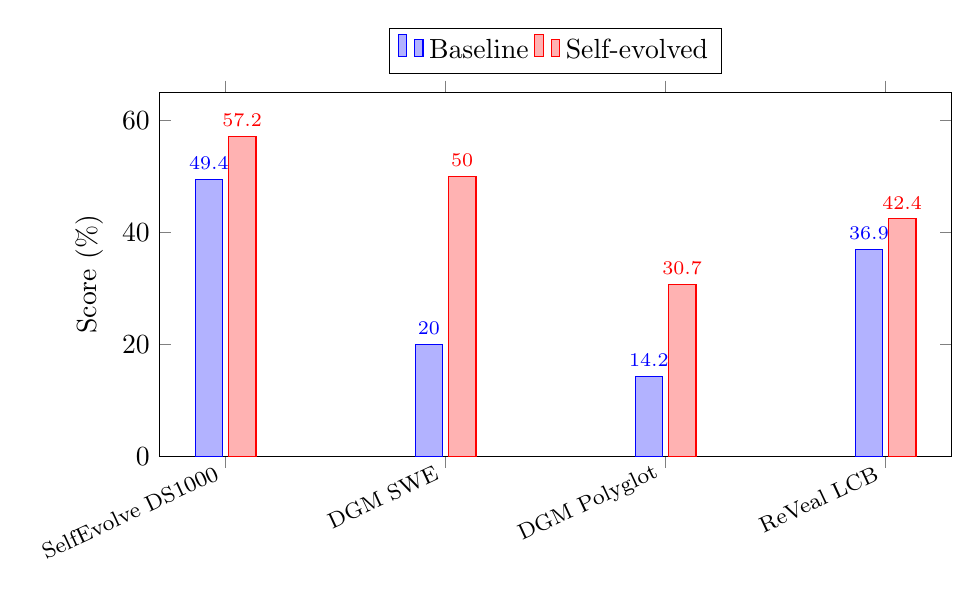
\begin{tikzpicture}
\begin{axis}[
    ybar,
    width=0.96\linewidth,
    height=6.2cm,
    ylabel={Score (\%)},
    symbolic x coords={SelfEvolve DS1000,DGM SWE,DGM Polyglot,ReVeal LCB},
    xtick=data,
    x tick label style={rotate=25,anchor=east,font=\footnotesize},
    ymin=0,
    ymax=65,
    legend style={at={(0.5,1.05)},anchor=south,legend columns=2},
    nodes near coords,
    nodes near coords style={font=\scriptsize},
]
\addplot coordinates {(SelfEvolve DS1000,49.4) (DGM SWE,20.0) (DGM Polyglot,14.2) (ReVeal LCB,36.9)};
\addplot coordinates {(SelfEvolve DS1000,57.2) (DGM SWE,50.0) (DGM Polyglot,30.7) (ReVeal LCB,42.4)};
\legend{Baseline,Self-evolved}
\end{axis}
\end{tikzpicture}
\caption{Representative code benchmark gains. The figure intentionally mixes benchmark families only to visualize gain magnitudes; the underlying tasks are not directly comparable.}
\label{fig:code-gains}
\end{figure}

The Reflexion result illustrates the promise and risk of iterative self-correction. On HumanEval, the agent receives feedback after failed attempts and stores reflection in memory. The reported 91.0\% pass@1 is striking, but the result should not be interpreted as a pure single-shot model capability. It is an agent-loop capability: generation, evaluation, reflection, memory, and retry. That distinction matters because a deployed coding system may care about final correctness, while a model-comparison leaderboard may care about first-attempt synthesis. Reflexion is therefore best read as evidence that verbal feedback can convert failed attempts into useful future context, not as evidence that the underlying model's raw coding ability changed.

SelfEvolve provides a different evaluation lesson. DS-1000 problems often fail because of API misuse, missing imports, shape errors, or library-version assumptions. SelfEvolve first asks the model to generate knowledge about the needed APIs and then executes candidate code in a sandbox. Error messages become revision signals. This makes DS-1000 a natural benchmark because the environment can produce informative feedback. The method's DS-1000 improvement from 49.4 to 57.2 is therefore not just a score; it demonstrates that executable traces can serve as a localized curriculum. The HumanEval pass@1 increase from 74.39 to 85.98 shows that the same broad principle transfers to simpler function synthesis, although GPT-4's 89.95 pass@1 baseline remains higher in the reported table.

DGM changes the unit of evaluation from a generated answer to an agent implementation. The system maintains an archive of agent variants, samples parent agents, asks a foundation model to modify agent code, evaluates the child on benchmarks, and retains improvements. The reported SWE-bench verified gain from 20.0\% to 50.0\% is therefore a process result over an evolving population. It should be evaluated not only by the final percentage but also by archive diversity, number of evaluated variants, failed modifications, compute budget, and transfer. The same method's Polyglot score increase from 14.2\% to 30.7\% suggests that the evolved agent improvements are not purely SWE-bench-specific, but transfer should be tested under frozen-agent conditions and with evaluator versioning.

ReVeal targets a weakness of many coding agents: they generate code more readily than they verify it. Its TAPO objective assigns credit at the turn level and explicitly optimizes self-verification. The LiveCodeBench result of 36.9 at turn 1 rising to 42.4 at turn 19 is important because it measures improvement across inference-time evolution rather than only across training updates. However, the number also demonstrates why efficiency reporting is essential. A turn-19 result has consumed much more computation than a turn-1 result. The right comparison depends on the application. For high-stakes code repair, a 5.5 point gain may justify many verifier turns. For latency-sensitive code completion, it may not.

SWE-bench and LiveCodeBench also expose two complementary threats. SWE-bench evaluates real repositories but can be sensitive to environment setup, flaky tests, and issue selection. LiveCodeBench reduces contamination through time-split problems but remains closer to contest programming than to long-term software maintenance. A strong code-evolution paper should therefore report both repository-level and time-split coding performance when possible. It should also include patch-quality metrics: number of files changed, test additions, dependency changes, lint errors, maintainability, and whether the patch solves the intended issue rather than merely satisfying tests.

For future code benchmarks, we recommend four additions. First, every self-evolution result should include a search budget: number of samples, turns, tests, tool calls, and wall-clock time. Second, benchmark harnesses should log whether generated tests were used for selection, because self-generated tests can become a source of Goodhart effects. Third, repository-level benchmarks should include unrelated regression tests and static analysis to detect broad damage. Fourth, benchmark reports should include negative candidate statistics: how often self-modifications failed to parse, failed tests, touched forbidden files, or reduced performance. Without these process statistics, code self-evolution cannot be compared scientifically.

\subsection{Mathematical Reasoning}
\label{subsec:mathematical-reasoning}

Mathematical reasoning is a second major evaluation domain because it offers crisp answers, rich reasoning traces, and, in formal settings, machine-checkable proofs. The common benchmarks are GSM8K, MATH, MiniF2F, and competition-math evaluations. GSM8K contains grade-school word problems with exact numeric answers \cite{gsm8k2021}. MATH contains more difficult high-school competition-style problems across algebra, geometry, number theory, counting, and precalculus \cite{math2021}. MiniF2F formalizes olympiad-level theorem statements across proof-assistant ecosystems and measures whether a system can produce a verified proof \cite{minif2f2021}. Competition-math evaluations include International Mathematical Olympiad (IMO) style scoring, where a system may be graded by solved problems or medal-equivalent point totals.

For self-evolution, mathematics has three attractive properties. First, many tasks have verifiable final answers, allowing reinforcement learning with verifiable rewards. Second, reasoning traces can be critiqued, revised, and distilled, making math a natural domain for self-refinement. Third, formal theorem proving provides a strong evaluator: a proof either checks or it does not. The difficulty is that informal math answers can be correct for the wrong reason, formalization can become the bottleneck, and public benchmarks have been heavily optimized by recent models.

Table~\ref{tab:math-exact-scores} summarizes reported numbers in the local corpus and related benchmark references. Self-Refine reports a math-reasoning accuracy increase from 56\% to 67\%. Agent Symbolic Learning reports MATH accuracy of 60.7\% with a GPT-4 backbone, compared with 56.0\% for the agent baseline and 48.4\% for DSPy in the same extracted table. RISE reports approximate GSM8K improvements from 14\% to 24\% for Llama2-7B and from 38\% to 46\% for Mistral-7B through learned recursive introspection. MiniF2F's original Lean GPT-f/PACT reference point is around 24.6\% pass@1 and 29.2\% pass@32 on the test split, while later expert-iteration and neural theorem-proving systems report higher cumulative pass rates. Competition-math systems such as AlphaGeometry and AlphaProof are not self-evolution systems in the narrow agentic sense, but they are relevant evaluation references because they use search, verification, and synthetic-data loops; AlphaGeometry solved 25 of 30 olympiad geometry problems, and the AlphaProof/AlphaGeometry combination solved 4 of 6 IMO 2024 problems, corresponding to a silver-medal-level result in public reporting \cite{alphageometry2024,alphaproof2024}.

\begin{table*}[t]
\centering
\small
\caption{Mathematical reasoning benchmark results relevant to self-evolution. Approximate values are marked with ``$\sim$'' when the source report gives rounded figures.}
\label{tab:math-exact-scores}
\begin{tabular}{p{0.18\linewidth}p{0.18\linewidth}p{0.20\linewidth}p{0.20\linewidth}p{0.14\linewidth}}
\toprule
\textbf{Method / reference} & \textbf{Benchmark} & \textbf{Baseline} & \textbf{Reported result} & \textbf{Metric} \\
\midrule
Self-Refine & Math reasoning task & 56\% & 67\% & Accuracy \\
Agent Symbolic Learning & MATH & Agents: 56.0\%; DSPy: 48.4\% & 60.7\% & Accuracy \\
RISE & GSM8K, Llama2-7B & $\sim$14\% single-turn & $\sim$24\% multi-turn introspection & Accuracy \\
RISE & GSM8K, Mistral-7B & $\sim$38\% single-turn & $\sim$46\% multi-turn introspection & Accuracy \\
MiniF2F reference & MiniF2F-test, Lean GPT-f/PACT & -- & 24.6\% pass@1; 29.2\% pass@32 & Verified proof rate \\
Expert iteration reference & MiniF2F-test & Prior GPT-f/PACT baseline & 29.6\% pass@1; 36.6\% pass@64 & Verified proof rate \\
AlphaGeometry & Olympiad geometry set & Previous symbolic/neural systems & 25 / 30 problems & Solved problems \\
AlphaProof + AlphaGeometry & IMO 2024 & Human competition scoring & 4 / 6 problems solved & Silver-level performance \\
\bottomrule
\end{tabular}
\end{table*}

The evaluation interpretation differs across the four benchmark families. GSM8K is useful for measuring arithmetic word-problem reliability, but it is vulnerable to answer-only shortcuts and contamination. MATH is harder and more diverse, but exact-answer grading can miss reasoning quality and can reward lucky final answers. MiniF2F is stricter because proof assistants verify the proof object, yet it moves part of the difficulty into formalization and search over proof tactics. IMO-style competition math is more meaningful to humans, but it is expensive to grade, small in sample size, and often not reproducible as a standardized benchmark.

Self-Refine's math result demonstrates that critique-and-rewrite can improve reasoning without weight updates. The method generates an answer, critiques its own output, and refines it. The increase from 56\% to 67\% shows that self-feedback can correct some errors, but the limitation is clear: if the model cannot identify the underlying mathematical mistake, it may refine a wrong solution into a more fluent wrong solution. This is why math evaluation should include intermediate checks when possible. A final answer can be correct by accident; a proof trace, symbolic derivation, or executable verification step provides stronger evidence.

RISE addresses a related issue by training the model to perform recursive introspection as a learned policy rather than as a prompt-only behavior. Its reported GSM8K gains for Llama2-7B and Mistral-7B indicate that the ability to decide when to revise can itself be optimized. The evaluation lesson is that multi-turn reasoning should be treated as a policy over compute allocation. A model that spends more introspection turns on difficult problems and fewer turns on easy problems may be more efficient than one with a fixed number of refinement rounds. Future math benchmarks should therefore report accuracy as a function of reasoning budget, not only a single final score.

Agent Symbolic Learning provides a bridge between math reasoning and agent evaluation. Its MATH result is not just a chain-of-thought prompt; it is the outcome of a symbolic optimization process over prompts, tools, and pipeline components. The extracted table reports 60.7\% accuracy with a GPT-4 backbone, above both the agent baseline and DSPy. This suggests that language-gradient updates can improve mathematical reasoning workflows. However, the comparison also raises a methodological concern: systems that optimize prompts on a benchmark must be evaluated on held-out tasks to distinguish true reasoning improvement from benchmark-specific prompt tuning.

MiniF2F and formal theorem proving are especially important for the next generation of self-evolution. A formal verifier provides a binary reward that is much harder to fool than a language-model judge. This makes theorem proving attractive for self-play, curriculum learning, and expert iteration. At the same time, formal proof systems expose a different kind of Goodhart risk: a prover may specialize in tactic patterns or formal-library artifacts rather than mathematical insight. Therefore, formal-math evaluation should report not only pass rates but also proof length, verifier calls, generated tactic diversity, dependence on imported lemmas, and performance on newly formalized problems.

Competition-math evaluation introduces an additional dimension: novelty and human-level problem solving. AlphaGeometry's 25/30 olympiad-geometry result and AlphaProof/AlphaGeometry's 4/6 IMO 2024 result show that search-and-verification systems can reach meaningful mathematical milestones. For the self-evolution literature, the significance is not that every agent should be evaluated on IMO problems. The significance is that mathematical discovery systems require evaluators that can certify nontrivial reasoning. If an evolving system claims to discover new lemmas, algorithms, or conjectures, it should provide proof artifacts, independent verification, or human-review protocols that go beyond answer matching.

A strong mathematical evaluation protocol should therefore include: (i) exact-answer benchmarks such as GSM8K for breadth; (ii) harder symbolic benchmarks such as MATH for depth; (iii) formal proof benchmarks such as MiniF2F for verification; (iv) time-split or newly generated tasks for contamination control; (v) compute-budget curves; and (vi) error taxonomy. Errors should be categorized as arithmetic slips, algebraic transformations, missing cases, false lemmas, invalid formalization, search failure, or evaluator mismatch. Self-evolution systems should then show which error categories decrease after evolution. A single aggregate accuracy hides whether the system learned mathematics or merely learned benchmark style.

\subsection{Agent Benchmarks}
\label{subsec:agent-benchmarks}

Agent benchmarks evaluate systems that act over multiple steps, often with tools, environments, memory, or external observations. They are crucial for AI self-evolution because many evolving systems are agents rather than pure text generators. The benchmark families considered here are HotPotQA for multi-hop question answering, ALFWorld for text-based embodied household tasks, WebArena for browser-based web tasks, and Minecraft environments such as Voyager for open-ended embodied skill acquisition.

HotPotQA evaluates multi-hop reasoning over documents and commonly reports exact match (EM) and F1 \cite{hotpotqa2018}. It is useful for testing whether an agent can decompose a question, retrieve or inspect evidence, and combine facts. ALFWorld maps household embodied tasks into a text environment where agents must issue actions to complete goals such as finding, moving, cleaning, heating, or cooling objects \cite{alfworld2020}. WebArena evaluates autonomous web agents across realistic websites such as shopping, forums, content management, and maps, with success measured by task completion \cite{webarena2023}. Voyager evaluates an open-ended Minecraft agent that writes, stores, and reuses skills, measuring exploration, technology-tree progress, and skill-library growth \cite{voyager2023}.

The main difference from code and math benchmarks is that agent benchmarks evaluate trajectories. The final answer may be less informative than the path. Did the agent use the right tool? Did it recover from errors? Did it take unnecessary actions? Did it persist unsafe memory? Did it overfit to a simulator? Did it transfer learned skills? For self-evolution, these questions are central because the evolving object may be the policy, prompt, tool-use pattern, memory, or skill library.

Table~\ref{tab:agent-exact-scores} summarizes exact reported numbers from the local corpus and widely cited benchmark reports. Agent Symbolic Learning reports HotPotQA F1/EM improvements from a baseline of 36.2/22.8 to 39.1/25.6, with DSPy at 37.4/24.1 in the extracted comparison. Reflexion reports ALFWorld success of 97\% versus a 75\% base success rate. WebArena's original benchmark showed that contemporary GPT-4 agents remained far below human performance, with a commonly cited GPT-4/ReAct-style success rate around 14.41\% compared with substantially higher human task completion. Voyager reports large open-ended Minecraft gains, including discovering 3.3 times more unique items, traveling 2.3 times longer distances, and unlocking key technology-tree milestones much faster than prior agents in its evaluation setting.

\begin{table*}[t]
\centering
\small
\caption{Agent benchmark results relevant to self-evolving systems. WebArena and Voyager numbers are included as environment references because they are central benchmarks for multi-step agent evaluation.}
\label{tab:agent-exact-scores}
\begin{tabular}{p{0.17\linewidth}p{0.17\linewidth}p{0.22\linewidth}p{0.24\linewidth}p{0.10\linewidth}}
\toprule
\textbf{Method} & \textbf{Benchmark} & \textbf{Baseline} & \textbf{Reported result} & \textbf{Metric} \\
\midrule
Agent Symbolic Learning & HotPotQA & Agents: F1 36.2, EM 22.8; DSPy: F1 37.4, EM 24.1 & F1 39.1, EM 25.6 & F1 / EM \\
Reflexion & ALFWorld & Base agent: 75\% & 97\% & Success rate \\
Godel Agent & HotPotQA / ALFWorld & Hand-designed agent baseline & Reported to exceed baselines; local extraction gives +8--15\% on HotPotQA and significant ALFWorld gains & Relative gain \\
WebArena reference & WebArena & Human performance far higher; early GPT-4 agents low & GPT-4/ReAct-style agents around 14.41\% in original benchmark reporting & Success rate \\
Voyager reference & Minecraft & Prior Minecraft agents & 3.3$\times$ unique items, 2.3$\times$ travel distance, faster tech-tree unlocking & Exploration/skill metrics \\
\bottomrule
\end{tabular}
\end{table*}

HotPotQA is a useful testbed for prompt and workflow evolution because errors often arise from poor decomposition or retrieval rather than missing world knowledge. Agent Symbolic Learning treats the agent as a symbolic network of prompts, tools, and pipeline connections. The evaluator constructs language losses from trajectories and propagates language gradients back through components. The HotPotQA gain from F1 36.2 to 39.1 and EM 22.8 to 25.6 is modest but meaningful because it indicates that structured prompt and pipeline updates can improve multi-hop behavior. The limitation is that HotPotQA is still mostly a question-answering benchmark; it does not fully test tool safety, long-term memory, or environment change.

ALFWorld adds sequential decision-making. Reflexion's 97\% success rate versus a 75\% base agent shows the value of memory-based verbal reinforcement in an environment where the agent can learn from failed episodes. The evaluation lesson is that episodic feedback can be highly effective when tasks repeat structural patterns. However, this also raises a transfer question: does the reflection memory capture general household strategies, or does it memorize environment-specific action patterns? A robust ALFWorld evaluation should include unseen task templates, randomized object locations, and memory ablation.

WebArena is important because it exposes the weakness of many LLM agents in realistic browser settings. Early GPT-4-based agents achieved only low double-digit success rates, around 14.41\% in the original benchmark setting, despite strong language ability. The gap reflects long-horizon planning, UI grounding, authentication state, form filling, error recovery, and website-specific affordances. For self-evolution, WebArena suggests that improving prompts alone may be insufficient. Systems may need better state representations, browser skill libraries, visual grounding, tool abstractions, and safe memory. Evaluation should report not only success but also invalid actions, page-navigation loops, timeouts, and whether the agent caused irreversible side effects.

Voyager represents a different kind of agent benchmark: open-ended skill acquisition rather than fixed task completion. The agent explores Minecraft, writes executable skills, stores them in a skill library, and reuses them for future tasks. Its reported gains of 3.3$\times$ unique items and 2.3$\times$ longer travel distance are not simple accuracy numbers. They measure coverage and exploration. This matters for self-evolution because open-ended agents should be evaluated by the growth of useful behavior, not only by success on a fixed checklist. At the same time, open-ended evaluation is hard: novelty can be shallow, exploration can be unsafe, and skill libraries can accumulate brittle or redundant code. Good evaluation should include skill reuse rate, skill correctness, dependency structure, and performance when the library is transferred to new worlds.

Agent benchmarks also need trajectory-level metrics. We recommend reporting: number of actions, invalid-action rate, recovery rate after failed tool calls, repeated-action loops, memory reads/writes, tool-call cost, human interventions, safety violations, and final success. For self-evolving agents, one should additionally report what changed between versions: prompt diff, memory diff, workflow diff, tool diff, or code diff. Without such diffs, a final success rate does not tell us what the system learned.

A particularly important evaluation issue is evaluator granularity. Binary task success can be too sparse for self-evolution. If an ALFWorld agent fails after twenty steps, the system needs to know whether it misunderstood the goal, chose the wrong object, failed to navigate, used the wrong action, or stopped too early. If a WebArena agent fails, the reason may be visual grounding, form validation, page state, login, or missing information. Process-oriented metrics convert failures into learning signals. This is why agent benchmarks should publish structured traces and failure taxonomies, not only final scores.

\subsection{Open-Ended Evaluation}
\label{subsec:open-ended-evaluation}

Open-ended self-evolution aims to discover artifacts that are not specified in advance: new algorithms, improved programs, novel proofs, better heuristics, or unexpected agent architectures. This is the evaluation regime of FunSearch, AlphaEvolve, DGM, ADAS, and AI Scientist-like systems. It is the most exciting regime because it moves beyond solving known tasks. It is also the hardest to evaluate because the evaluator must distinguish genuine novelty from overfitting, rediscovery, or benchmark gaming.

FunSearch uses a language model to generate programs and an evaluator to score them, iterating over a database of high-scoring candidate programs. It demonstrated new constructions for the cap set problem and improved heuristics for online bin packing \cite{funsearch2023}. AlphaEvolve generalizes the idea to larger codebases and combines Gemini Flash for broad exploration with Gemini Pro for deeper candidate generation, using an evolutionary database and quality-diversity search. The local paper summary reports several headline results: a 4$\times$4 complex matrix multiplication algorithm using 48 multiplications, described as the first improvement over Strassen-style results in 56 years for that setting; rediscovery of state-of-the-art solutions for 75\% of more than 50 mathematical problems and improvement beyond known best results for 20\%; recovery of 0.7\% of worldwide compute in Google's Borg scheduling context; a 23\% speedup in one LLM-training kernel-tiling setting; and a 32\% speedup in another attention-related optimization setting.

\begin{table*}[t]
\centering
\small
\caption{Open-ended discovery results from FunSearch and AlphaEvolve-style systems. These results require evaluators that certify candidate quality rather than merely compare against a fixed answer key.}
\label{tab:open-ended-results}
\begin{tabular}{p{0.18\linewidth}p{0.30\linewidth}p{0.34\linewidth}p{0.10\linewidth}}
\toprule
\textbf{System} & \textbf{Domain} & \textbf{Reported result} & \textbf{Evaluator} \\
\midrule
FunSearch & Cap set / extremal combinatorics & Discovered new high-scoring constructions beyond previously known programmatic baselines & Objective combinatorial score \\
FunSearch & Online bin packing & Found improved heuristics for bin-packing variants & Simulation score \\
AlphaEvolve & 4$\times$4 complex matrix multiplication & 48 multiplications; reported as first improvement in 56 years for the target setting & Algebraic verification / program evaluator \\
AlphaEvolve & 50+ mathematical problems & Re-discovered SOTA for 75\%; improved best known for 20\% & Problem-specific evaluators \\
AlphaEvolve & Borg scheduling & Recovered 0.7\% of worldwide compute & Production scheduling evaluator \\
AlphaEvolve & LLM training kernels & 23\% speedup in kernel tiling; 32\% speedup in another attention optimization & Runtime benchmark \\
AI Scientist v2 & Automated paper generation & Peer-review score 6.33; top 45\% workshop-level ranking & Human/LLM peer review \\
\bottomrule
\end{tabular}
\end{table*}

The key evaluation challenge in open-ended discovery is novelty. A system may rediscover a known result, improve a benchmark-specific heuristic, or find a genuine new contribution. These outcomes should be reported separately. Rediscovery is valuable because it validates the search process, but it is not the same as discovery. Improvement on a synthetic evaluator is valuable if the evaluator matches the real problem, but it may not transfer. Genuine discovery requires independent verification, comparison with the literature, and often expert review.

AlphaEvolve's results show why open-ended evaluation must include domain-specific validators. Matrix multiplication improvements require algebraic correctness, not judge-model preference. Scheduling improvements require production-like simulators or shadow deployments, not a language explanation. Kernel speedups require hardware-specific runtime measurements with noise control. Mathematical-problem improvements require proof or exhaustive verification. A single generic benchmark cannot evaluate all these outputs. Open-ended self-evolution therefore needs evaluator portfolios: each domain must define a reliable scoring function, a novelty check, and an independent validation path.

FunSearch also demonstrates the importance of interpretable artifacts. The generated object is a program, not just a number. Humans can inspect the program, simplify it, connect it to known theory, and sometimes extract a mathematical insight. This is a strength of program-search approaches. If an LLM only outputs a final score or opaque solution, discovery is harder to validate. For self-evolution, executable and inspectable artifacts should be preferred because they support verification, reuse, and scientific understanding.

Open-ended evaluation should include archive metrics. A population or database is not merely an implementation detail; it is part of the system's intelligence. Useful metrics include number of unique niches filled, best score over time, median score over time, novelty of accepted candidates, lineage depth, proportion of candidates that compile or verify, rediscovery rate, and diversity of strategies. Quality-diversity methods such as MAP-Elites explicitly optimize a map of elites across behavioral descriptors. Reporting only the single best artifact discards much of the evidence about the search process.

Open-ended systems also require negative-result reporting. If AlphaEvolve improves 20\% of more than 50 mathematical problems, what happened on the remaining problems? Did it fail to generate valid candidates, rediscover known solutions, overfit the evaluator, or find no improvement? If FunSearch works on cap sets and bin packing, what domains did not work? Failure taxonomy is essential because open-ended discovery is expensive. Practitioners need to know which evaluator properties make a domain suitable: cheap scoring, dense feedback, reliable verification, decomposable artifacts, and enough room for improvement.

AI Scientist illustrates a different open-ended evaluation problem: evaluating scientific artifacts rather than programs. The local corpus reports that AI Scientist v1 generated papers across diffusion models, language modeling, and grokking at approximately \$15 per paper, while AI Scientist v2 achieved a peer-review score of 6.33 and top-45\% workshop-level ranking. These numbers are important, but peer review is noisy and can be gamed by fluent writing. Independent evaluation found limitations such as rejection of human-accepted papers, weak generalization, limited theoretical depth, and restricted architectural diversity. This case shows that open-ended evaluation must combine automated reviewers with human experts, novelty search over literature, reproducibility checks, and artifact-level validation.

A good open-ended evaluation protocol should therefore require: (i) a precise objective or validator; (ii) an explicit novelty check against known results; (iii) reproducibility artifacts; (iv) archive and search-budget statistics; (v) independent expert or formal verification for claimed discoveries; (vi) failure taxonomy; and (vii) a distinction between rediscovery, benchmark improvement, and new knowledge. Without these layers, open-ended self-evolution risks becoming a generator of impressive anecdotes rather than cumulative science.

\subsection{Star Quality Analysis}
\label{subsec:star-quality-analysis}

Research benchmarks measure technical capability, but the Self Evolve ecosystem also needs to evaluate project quality. GitHub stars are a noisy signal: they measure attention, not necessarily reliability, maintainability, or research value. The star-analysis report in the source materials therefore proposes a quality scoring system that combines star activity, contributor diversity, fork quality, issue quality, and pull-request merge rate. This section incorporates that 12-project ranking and interprets it as an ecosystem-level evaluation tool.

The report's key conclusion is that raw stars can invert quality. AutoGPT has approximately 175,000 stars but receives a composite quality score of only 28/100. OpenEvolve has approximately 6,358 stars but receives the highest composite score, 74/100. DSPy, SWE-Agent, OpenHands, LangGraph, AutoGen, FunSearch, CrewAI, Reflexion, MetaGPT, AutoGPT, and Devika form the 12-project ranking shown in Table~\ref{tab:star-ranking}. The analysis identifies Stars/Contributor ratio as a particularly useful hype detector: below 50 is healthy, 50--150 warrants attention, and above 150 is high-risk. AutoGPT's Stars/Contributor ratio is reported as 213, while Devika's is 183, both above the suspicious threshold. CrewAI's 107 is in the watch range but supported by steadier growth and stronger community health.

\begin{table*}[t]
\centering
\small
\caption{Twelve-project GitHub quality ranking from \texttt{reports/star-analysis-report.md}. The composite score averages star activity, contributor diversity, fork quality, issue quality, and PR merge rate.}
\label{tab:star-ranking}
\begin{tabular}{r p{0.18\linewidth} r r p{0.16\linewidth} p{0.24\linewidth}}
\toprule
\textbf{Rank} & \textbf{Project} & \textbf{Stars} & \textbf{Score} & \textbf{Growth} & \textbf{Interpretation} \\
\midrule
1 & OpenEvolve & 6,358 & 74 & organic & High-quality niche project \\
2 & DSPy & 25,000 & 73 & organic & Strong academic and engineering signal \\
3 & SWE-Agent & 15,000 & 70 & organic & ICLR Oral endorsement and strong benchmark focus \\
4 & OpenHands & 55,000 & 68 & organic & Highest community-health profile among large projects \\
5 & LangGraph & 20,000 & 67 & steady & Solid architecture and ecosystem fit \\
6 & AutoGen & 50,000 & 66 & organic & Microsoft-backed multi-agent framework \\
7 & FunSearch & 1,500 & 62 & organic & Under-starred but high-quality research project \\
8 & CrewAI & 30,000 & 62 & steady & Practical community adoption with manageable hype risk \\
9 & Reflexion & 3,158 & 58 & steady & Classic research implementation \\
10 & MetaGPT & 50,000 & 56 & viral & Academic/commercial balance but media-amplified growth \\
11 & AutoGPT & 175,000 & 28 & viral & Hype-driven; raw stars overstate quality \\
12 & Devika & 22,000 & 30 & suspicious & Me-too growth pattern tied to Devin attention \\
\bottomrule
\end{tabular}
\end{table*}

The scoring formula is simple but useful:
\begin{equation}
\mathrm{CompositeScore}=0.20 S_{activity}+0.20 C_{diversity}+0.20 F_{quality}+0.20 I_{quality}+0.20 P_{merge}.
\end{equation}
Here $S_{activity}$ measures the share of recent active stargazers, $C_{diversity}$ reverses contributor concentration, $F_{quality}$ estimates the fraction of forks with meaningful commits, $I_{quality}$ measures non-spam issue quality, and $P_{merge}$ is merged pull requests divided by total pull requests. The equal weighting is not definitive, but it is transparent. A project can no longer hide behind raw stars if forks are empty, issues are repetitive, contributors are concentrated, and pull requests are rarely merged.

\begin{figure}[t]
\centering
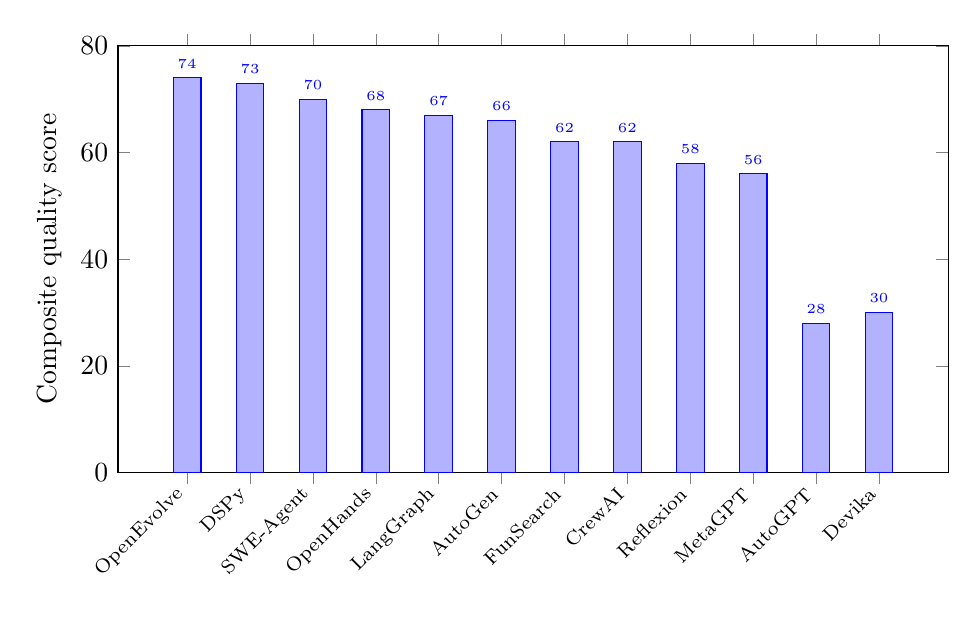
\begin{tikzpicture}
\begin{axis}[
    ybar,
    width=\linewidth,
    height=7cm,
    ylabel={Composite quality score},
    symbolic x coords={OpenEvolve,DSPy,SWE-Agent,OpenHands,LangGraph,AutoGen,FunSearch,CrewAI,Reflexion,MetaGPT,AutoGPT,Devika},
    xtick=data,
    x tick label style={rotate=45,anchor=east,font=\scriptsize},
    ymin=0,
    ymax=80,
    nodes near coords,
    nodes near coords style={font=\tiny},
]
\addplot coordinates {(OpenEvolve,74) (DSPy,73) (SWE-Agent,70) (OpenHands,68) (LangGraph,67) (AutoGen,66) (FunSearch,62) (CrewAI,62) (Reflexion,58) (MetaGPT,56) (AutoGPT,28) (Devika,30)};
\end{axis}
\end{tikzpicture}
\caption{Composite star-quality ranking. The figure shows that raw popularity and ecosystem quality can diverge sharply.}
\label{fig:star-quality}
\end{figure}

The report reconstructs propagation chains that explain why raw stars can mislead. AutoGPT grew from creation on March 30, 2023 to approximately 50,000 stars by April 2 after Twitter/X demonstrations, Elon Musk amplification, Hacker News and Reddit exposure, YouTube tutorials, and translated media coverage. The report classifies this as hype-driven growth: fast rise, high Stars/Contributor ratio, many inactive stargazers, and repetitive issues. Devika shows a similar but more derivative pattern: it was framed as an open-source Devin alternative, reached around 20,000 stars within days, and then suffered steep activity decline. By contrast, DSPy, SWE-Agent, OpenEvolve, and FunSearch show slower academic or engineering-driven adoption.

Star quality matters for AI self-evolution because the field is tool-heavy. Practitioners often choose frameworks, agents, memory systems, evaluators, and code-evolution platforms based on GitHub visibility. If raw stars dominate selection, teams may adopt projects that are popular but poorly maintained. A quality-adjusted ranking helps distinguish durable infrastructure from social-media spikes. It also helps identify underappreciated research artifacts. FunSearch's 1,500 stars and score of 62 suggest that scientific value may be high even when community size is small. OpenEvolve's top score suggests that a focused implementation of AlphaEvolve-like ideas can be more trustworthy than a viral general-purpose agent.

The star-quality framework should be treated as a complement to technical benchmarks, not a replacement. A project can have excellent benchmark results and poor community health, or strong community health and weak research novelty. For production adoption, both matter. A self-evolution system should be evaluated by capability, maintainability, documentation, issue responsiveness, contributor diversity, security posture, and licensing. The star-quality score provides an initial signal for maintainability and community health.

There are limitations. GitHub API-derived measures can be noisy. Fork quality requires deeper analysis than fork count. Issue quality may require language-specific NLP and can be biased against non-English communities. PR merge rate can be low for healthy projects that use internal development or strict review. Stars/Contributor ratio can penalize mature projects with large user bases. Therefore, the framework should not be used as a mechanical ranking. It should be used as an audit checklist: if raw stars are high but contributor diversity, fork quality, issue quality, and PR merge rate are low, investigate before adopting.

For future ecosystem reports, we recommend adding dependency health, release cadence, security advisories, test coverage, documentation freshness, benchmark reproducibility, and maintainer bus factor. Self-evolution projects are especially sensitive to evaluator and sandbox quality; a project with unsafe defaults can create real risk even if it is popular. Star quality should therefore be integrated with safety and reproducibility audits.

\subsection{Process-Oriented Metrics}
\label{subsec:process-oriented-metrics}

Static benchmark scores answer the question, ``How good is the final system?'' Process-oriented metrics answer the question, ``How did the system improve, and can that improvement be trusted?'' For self-evolution, process metrics are essential because the path is part of the method. A system that improves smoothly over many validated iterations is different from one that finds a lucky candidate after many failures. A system that maintains diverse archives is different from one that collapses to a brittle local optimum. A system whose improvement transfers is different from one that overfits to a single evaluator.

\paragraph{Iteration gain curves.}
The first process metric is the gain curve: score as a function of iteration, turn, candidate count, or cost. Let $s_t$ be the validation or held-out score after iteration $t$. The marginal gain is
\begin{equation}
\Delta_t = s_t - s_{t-1}.
\end{equation}
The cumulative gain is $s_T-s_0$, and the gain efficiency can be normalized by cost $c_t$:
\begin{equation}
\eta_T = \frac{s_T-s_0}{\sum_{t=1}^{T} c_t}.
\end{equation}
Gain curves reveal saturation, instability, and regressions. For example, ReVeal's LiveCodeBench curve from turn 1 to turn 19 shows inference-time improvement but should be accompanied by per-turn cost. DGM's archive evolution should show best score, median score, and accepted-candidate count over iterations. Self-Refine-style systems should show whether most improvement occurs in the first refinement or continues across later rounds.

\paragraph{Regression curves.}
Improvement on a target benchmark may hide degradation elsewhere. Let $R_t$ be a regression-suite score after update $t$. A safe update should satisfy both $s_t > s_{t-1}$ and $R_t \geq R_{t-1}-\epsilon$ for an acceptable tolerance $\epsilon$. In production, regression suites should include safety tests, previous user tasks, cost limits, latency, and tool-permission tests. A candidate update that improves HumanEval while increasing unsafe file edits should be rejected.

\paragraph{Archive diversity.}
Population-based systems such as DGM and AlphaEvolve require archive metrics. If the archive contains $n$ artifacts with behavioral descriptors $b_i$, one simple diversity metric is average pairwise distance:
\begin{equation}
D(A)=\frac{2}{n(n-1)}\sum_{i<j} d(b_i,b_j).
\end{equation}
For code agents, descriptors may include tool-use patterns, edit strategies, prompt templates, test-generation behavior, or module-level changes. For program discovery, descriptors may include algorithmic structure, runtime profile, proof strategy, or mathematical construction family. Diversity matters because open-ended progress often depends on stepping stones that are not immediately best on the main objective.

\paragraph{Lineage and stepping-stone metrics.}
An archive should record parent-child relationships. Useful metrics include lineage depth, branching factor, number of ancestors contributing to the best artifact, and time between stepping stones. A best artifact that descends from many modest improvements provides different evidence than one found by random sampling. Lineage also supports interpretability: researchers can inspect which modifications mattered.

\paragraph{Transfer metrics.}
Let $S_{A\rightarrow A}$ be performance after evolving on source domain $A$ and evaluating on $A$, and let $S_{A\rightarrow B}$ be performance after evolving on $A$ but evaluating on target domain $B$ without further adaptation. A simple transfer ratio is
\begin{equation}
T_{A\rightarrow B}=\frac{S_{A\rightarrow B}-S_{0\rightarrow B}}{S_{A\rightarrow A}-S_{0\rightarrow A}+\delta},
\end{equation}
where $S_0$ is the seed system and $\delta$ avoids division by zero. A high transfer ratio indicates reusable improvement. A low or negative ratio indicates overfitting or harmful specialization. Transfer should be measured across benchmarks, languages, task types, environments, model backbones, and time splits.

\paragraph{Evaluator sensitivity.}
Self-evolution can overfit to evaluator quirks. Evaluator sensitivity measures how rankings change under alternative evaluators. If candidate $a_i$ is best under evaluator $E_1$ but poor under $E_2$, the improvement may be fragile. Researchers can report rank correlation between evaluators, disagreement rate, and score variance across evaluator seeds. For LLM judges, evaluator sensitivity should include different model families and prompt variants. For code tests, it should include hidden tests, mutation tests, and property-based tests.

\paragraph{Cost-normalized improvement.}
Cost-normalized metrics should be first-class. A practical score might be
\begin{equation}
\mathrm{Utility}=\mathrm{CorrectnessGain}-\lambda_1\mathrm{Cost}-\lambda_2\mathrm{Latency}-\lambda_3\mathrm{Risk}-\lambda_4\mathrm{HumanBurden}.
\end{equation}
The coefficients depend on the deployment setting, but the structure is universal. An evolving system is useful when its marginal gain exceeds the marginal cost and risk. Papers should report enough raw data for readers to compute their own utility under different assumptions.

\paragraph{Memory quality metrics.}
For memory-based self-evolution, process metrics should include memory precision, memory recall, stale-memory rate, contradiction rate, retrieval utility, and memory write acceptance. A reflection that is never retrieved is wasted. A reflection that is retrieved in the wrong context is harmful. A memory store that grows without consolidation increases cost and drift risk. Longitudinal memory benchmarks should measure whether the agent improves over sessions without accumulating misleading lessons.

\paragraph{Safety-process metrics.}
Safety should also be process-oriented. Count candidate updates rejected for safety reasons, sandbox violations, attempts to access forbidden resources, evaluator modification attempts, rollback events, and human escalations. These metrics should not be hidden as embarrassing failures; they are evidence that the safety gate is doing work. A system with zero reported safety events may be safe, or it may simply lack instrumentation.

Process-oriented evaluation changes how results are interpreted. A final score is a point estimate. A process report is a trajectory. For self-evolution, the trajectory is often the scientific contribution. It shows whether improvement is monotonic, whether diversity is preserved, whether cost explodes, whether transfer emerges, and whether safety gates catch bad candidates. Future benchmarks should therefore require trace submissions, not just final answers.

\subsection{Recommended Evaluation Protocol}
\label{subsec:recommended-evaluation-protocol}

We conclude with an eight-point checklist for evaluating AI self-evolution systems. The checklist is designed for papers, open-source projects, and production pilots. It is intentionally stricter than conventional model benchmarking because self-evolution introduces additional degrees of freedom.

\paragraph{1. Define the evolving object.}
State exactly what changes: output only, prompt, memory, tool description, workflow graph, code, archive, reward model, or model weights. Many ambiguities disappear when the evolving object is explicit. A method that revises an answer is different from a method that rewrites its own source code.

\paragraph{2. Freeze and document the evaluator.}
Record benchmark version, task split, hidden-test policy, judge prompts, environment versions, tool versions, random seeds, and scoring scripts. If the evaluator changes during the experiment, report evaluator lineage. The agent should not be able to modify the evaluator unless evaluator evolution is the object of study and is separately audited.

\paragraph{3. Report the adaptation budget.}
Include number of turns, samples, candidates, tool calls, tests, environment steps, verifier calls, tokens, wall-clock time, API cost, GPU time, and human review minutes. Separate training-time, validation-time, and inference-time budgets. Do not compare a turn-20 result to a single-shot baseline without budget normalization.

\paragraph{4. Use train--validation--test separation for evolution.}
Candidate updates may be selected on training or validation tasks, but final claims should use held-out tasks. For time-sensitive domains, use time splits. For repository tasks, use repositories not seen during prompt or workflow tuning. For memory systems, test on sessions not used for memory construction.

\paragraph{5. Measure regressions and safety constraints.}
Maintain a regression suite that includes previous capabilities, safety policies, cost limits, latency, forbidden actions, privacy constraints, and rollback tests. Reject updates that improve the main benchmark while violating constraints. Report rejected updates and reasons.

\paragraph{6. Evaluate transfer and robustness.}
Freeze the evolved artifact and test it on new domains, seeds, paraphrases, environments, tools, model backbones, or time periods. Report confidence intervals and sensitivity to evaluator variants. Include perturbation tests for memory, prompts, and tool failures.

\paragraph{7. Publish process traces and archive statistics.}
For iterative systems, publish gain curves, candidate counts, accepted/rejected updates, archive diversity, lineage, and negative results. For privacy or safety reasons, traces may be redacted, but the structure should remain available. A self-evolution method without process evidence is hard to reproduce.

\paragraph{8. Normalize by cost and operational value.}
Report improvement per dollar, per token, per verifier call, per wall-clock hour, and per human review minute. Include maintenance burden and deployment constraints. A benchmark gain is not sufficient if the required cost, risk, or operational complexity exceeds the value of the improvement.

\begin{table*}[t]
\centering
\small
\caption{Eight-point protocol for evaluating self-evolution systems.}
\label{tab:eight-point-protocol}
\begin{tabular}{p{0.06\linewidth}p{0.24\linewidth}p{0.56\linewidth}}
\toprule
\textbf{No.} & \textbf{Protocol item} & \textbf{Minimum evidence} \\
\midrule
1 & Evolving object & Explicit artifact type and allowed update operators. \\
2 & Frozen evaluator & Benchmark version, splits, scripts, judge prompts, environment, seeds. \\
3 & Adaptation budget & Turns, candidates, samples, tools, tokens, wall-clock, dollars, human minutes. \\
4 & Held-out testing & Train/validation/test or time-split separation; no final selection on test. \\
5 & Regression and safety & Regression suite, forbidden actions, rollback, rejected update statistics. \\
6 & Transfer and robustness & Cross-domain tests, perturbations, confidence intervals, evaluator sensitivity. \\
7 & Process traces & Gain curves, archive metrics, lineage, negative candidates, trace schema. \\
8 & Cost-normalized value & Gain per resource unit and operational utility analysis. \\
\bottomrule
\end{tabular}
\end{table*}

The checklist can be used as a scoring rubric. A minimal demonstration may satisfy only items 1--3. A publishable benchmark paper should satisfy items 1--7. A production-ready self-evolution system should satisfy all eight and add security review, access control, incident response, and monitoring. The key is not bureaucracy; it is epistemic hygiene. Self-evolution systems are optimization processes. Optimization processes exploit whatever signal they receive. Evaluation must therefore be designed as a robust control system, not as an afterthought.

Across the benchmarks reviewed in this chapter, the most reliable gains appear where feedback is executable, independent, and cheap: code tests, theorem provers, simulators, and domain-specific evaluators. The least reliable claims appear where evaluation depends on vague judge preference, raw popularity, or unreported search budgets. The field's next step is not to abandon benchmarks, but to make them harder to game and richer in process evidence. Correctness, efficiency, transfer, robustness, safety, and cost must be reported together. Only then can AI self-evolution move from impressive improvement anecdotes to cumulative, trustworthy science.
